\documentclass[../main.tex]{subfiles}

\begin{document}

\subsubsection*{2\hfill}
We have the following language over the alphabet $\Sigma = \{a, b\}$
\begin{equation*}
	A = \{w | w \text{ ends with } \mathbf{ba}\}
\end{equation*}
\begin{enumerate}[a)]
	\item Draw a state diagram for a DFA which recognizes $A$.
	\item Express $A$ using a regular expression.
	\item Find a regular grammar that generates $A$.
	\item We have the following language over the alphabet $\Sigma = \{a, b\}$
		\begin{equation*}
			B = \{w | w \text{ contains an odd number of } \mathbf{b} \text{ or more than one } \mathbf{a}\}
		\end{equation*}
		Draw a state diagram for a DFA which recognizes $B$.
\end{enumerate}

\solution
\begin{enumerate}[a)]
	\item 
	\item 
	\item 
	\item 
	\item 
\end{enumerate}

\begin{enumerate}[a)]
    \item\begin{center}
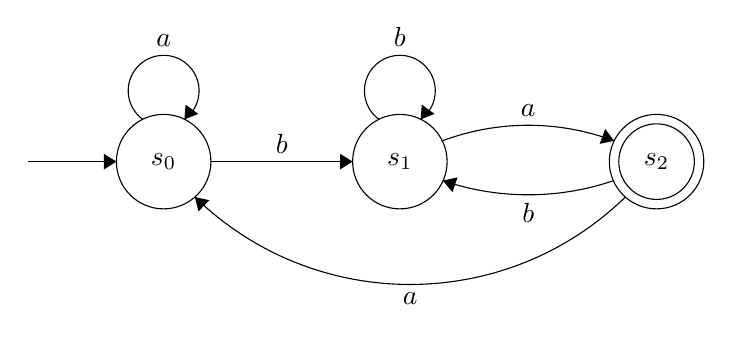
\begin{tikzpicture}[scale=0.2]
\tikzstyle{every node}+=[inner sep=0pt]
\draw [black] (13,-20.2) circle (3);
\draw (13,-20.2) node {$s_0$};
\draw [black] (28,-20.2) circle (3);
\draw (28,-20.2) node {$s_1$};
\draw [black] (44.3,-20.2) circle (3);
\draw (44.3,-20.2) node {$s_2$};
\draw [black] (44.3,-20.2) circle (2.4);
\draw [black] (4.4,-20.2) -- (10,-20.2);
\fill [black] (10,-20.2) -- (9.2,-19.7) -- (9.2,-20.7);
\draw [black] (11.677,-17.52) arc (234:-54:2.25);
\draw (13,-12.95) node [above] {$a$};
\fill [black] (14.32,-17.52) -- (15.2,-17.17) -- (14.39,-16.58);
\draw [black] (16,-20.2) -- (25,-20.2);
\fill [black] (25,-20.2) -- (24.2,-19.7) -- (24.2,-20.7);
\draw (20.5,-19.7) node [above] {$b$};
\draw [black] (30.69,-18.882) arc (110.58037:69.41963:15.534);
\fill [black] (41.61,-18.88) -- (41.04,-18.13) -- (40.69,-19.07);
\draw (36.15,-17.39) node [above] {$a$};
\draw [black] (41.56,-21.412) arc (-71.24018:-108.75982:16.823);
\fill [black] (30.74,-21.41) -- (31.34,-22.14) -- (31.66,-21.2);
\draw (36.15,-22.81) node [below] {$b$};
\draw [black] (26.677,-17.52) arc (234:-54:2.25);
\draw (28,-12.95) node [above] {$b$};
\fill [black] (29.32,-17.52) -- (30.2,-17.17) -- (29.39,-16.58);
\draw [black] (42.318,-22.448) arc (-45.77785:-134.22215:19.598);
\fill [black] (14.98,-22.45) -- (15.21,-23.36) -- (15.9,-22.65);
\draw (28.65,-28.5) node [below] {$a$};
\end{tikzpicture}
\end{center} 

    \item $(a \cup b)^\ast ba$

    \item 

    \item \begin{center}
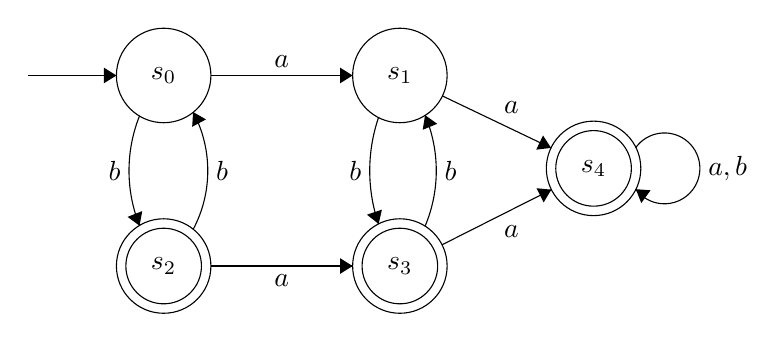
\begin{tikzpicture}[scale=0.2]
\tikzstyle{every node}+=[inner sep=0pt]
\draw [black] (13,-20.2) circle (3);
\draw (13,-20.2) node {$s_0$};
\draw [black] (28,-20.2) circle (3);
\draw (28,-20.2) node {$s_1$};
\draw [black] (13,-32.3) circle (3);
\draw (13,-32.3) node {$s_2$};
\draw [black] (13,-32.3) circle (2.4);
\draw [black] (28,-32.3) circle (3);
\draw (28,-32.3) node {$s_3$};
\draw [black] (28,-32.3) circle (2.4);
\draw [black] (40.3,-26.1) circle (3);
\draw (40.3,-26.1) node {$s_4$};
\draw [black] (40.3,-26.1) circle (2.4);
\draw [black] (4.4,-20.2) -- (10,-20.2);
\fill [black] (10,-20.2) -- (9.2,-19.7) -- (9.2,-20.7);
\draw [black] (16,-20.2) -- (25,-20.2);
\fill [black] (25,-20.2) -- (24.2,-19.7) -- (24.2,-20.7);
\draw (20.5,-19.7) node [above] {$a$};
\draw [black] (11.468,-29.735) arc (-158.2819:-201.7181:9.418);
\fill [black] (11.47,-29.74) -- (11.64,-28.81) -- (10.71,-29.18);
\draw (10.3,-26.25) node [left] {$b$};
\draw [black] (14.871,-22.522) arc (28.02661:-28.02661:7.934);
\fill [black] (14.87,-22.52) -- (14.81,-23.46) -- (15.69,-22.99);
\draw (16.3,-26.25) node [right] {$b$};
\draw [black] (16,-32.3) -- (25,-32.3);
\fill [black] (25,-32.3) -- (24.2,-31.8) -- (24.2,-32.8);
\draw (20.5,-32.8) node [below] {$a$};
\draw [black] (29.598,-22.723) arc (22.87238:-22.87238:9.074);
\fill [black] (29.6,-22.72) -- (29.45,-23.65) -- (30.37,-23.27);
\draw (30.81,-26.25) node [right] {$b$};
\draw [black] (26.645,-29.635) arc (-161.22603:-198.77397:10.517);
\fill [black] (26.65,-29.63) -- (26.86,-28.72) -- (25.91,-29.04);
\draw (25.59,-26.25) node [left] {$b$};
\draw [black] (30.7,-21.5) -- (37.6,-24.8);
\fill [black] (37.6,-24.8) -- (37.09,-24.01) -- (36.66,-24.91);
\draw (35.08,-22.64) node [above] {$a$};
\draw [black] (30.68,-30.95) -- (37.62,-27.45);
\fill [black] (37.62,-27.45) -- (36.68,-27.36) -- (37.13,-28.26);
\draw (35.09,-29.7) node [below] {$a$};
\draw [black] (42.98,-24.777) arc (144:-144:2.25);
\draw (47.55,-26.1) node [right] {$a,b$};
\fill [black] (42.98,-27.42) -- (43.33,-28.3) -- (43.92,-27.49);
\end{tikzpicture}
\end{center}
\end{enumerate}

\end{document}
